
% Computer Architecture (4190.308) Fall 2016 
% Seoul National University CARES Lab
% Lab 1 documentation

% Lines that need modification : 29~31, 96~100, 105~109

\documentclass{article}
\usepackage{graphicx, caption, subcaption, verbatim, moreverb, alltt, kotex}
\usepackage[protrusion=true,expansion=true]{microtype}
\usepackage{fancyvrb}
\usepackage{hhline}
\usepackage{multirow}
\let\verbatiminput=\verbatimtabinput

\setlength{\oddsidemargin}{0.25in}	% 1.25in left margin
\setlength{\evensidemargin}{0.25in}	% 1.25in left margin (even pages)
\setlength{\topmargin}{0.0in}		% 1in top margin
\setlength{\textwidth}{6.0in}		% 6.0in text - 1.25in rt margin
\setlength{\textheight}{9in}		% Body ht for 1in margins
\addtolength{\topmargin}{-\headheight}	% No header, so compensate
\addtolength{\topmargin}{-\headsep}	% for header height and separation


% type user-defined commands here

\begin{document}

\title{Lab 1: Combinational Circuits}   % type title between braces
\author{CSE 4190.308 Computer Architecture \\ 5 Exercises (Total 60 Points)}
\date{Received: March 12, 2016 \\Due: 11:00 a.m., March 21, 2016\\ \ \\ TA Office Hours: 7:00 - 8:00 p.m., 3/18, 3/19, 3/20}
\maketitle

\section{Introduction}

You will build up a barrel shifter from gate primitives. First, you will build a
1-bit multiplexer. Next, you will write a polymorphic multiplexer
using for-loops. Using the gate-level multiplexer function, you will then
construct a combinational barrel-shifter. Finally, we will add a simple
gate-level modification to the barrel shifter to support the arithmetic right
shift operation. This allows us to use the barrel shifter for both logical and
arithmetic operations.

The left shift (\verb|<<|) and right shift (\verb|>>|) operations are employed in computer
programs to manipulate bits and to simplify multiplication and division in some
special cases. Shifting is considered a simple operation because shift has a
relatively small and fast implementation in hardware; shift can typically be
implemented in a single processor cycle, while multiplication and division take
multiple cycles.

Shifts are inexpensive in hardware because their functional implementation
involves wiring, rather than transistors. For example, a shift by a constant
value is implemented with wires, as shown in Figure~\ref{fig:wired_shifter}. Variable
Shifting is more complicated, but still efficient.

The barrel shifter (shown in Figure~\ref{fig:variable_shifter}) is more general
than the wired shifter, but requires more hardware. The shift amount
(\texttt{shiftAmt}) determines how far the input is shifted.

The microarchitecture of the barrel shifter is a logarithmic circuit for
variable length shifting. The key observation in this microarchitecture is that
any shift can be done by applying a sequence of smaller shifts. For example, a
left shift by three can be decomposed into a shift by one and a shift by two. At
each level of the shifter, the shifter conditionally shifts the data, using a
multiplexer to select the data for the next stage.


In this lab we will implement the right shift operation, for which there are two
possible meanings, logical and arithmetic which differ in preservation of the
two's complement sign bit.

\begin{figure}
\centering
\begin{subfigure}[b]{0.49\textwidth}
	\centering
	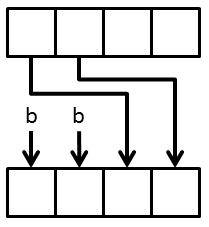
\includegraphics[width=0.5\linewidth]{WiredShifter.png}
	\caption{Wired Shifting by a Constant Value}
	\label{fig:wired_shifter}
\end{subfigure}
\begin{subfigure}[b]{0.49\textwidth}
	\centering
	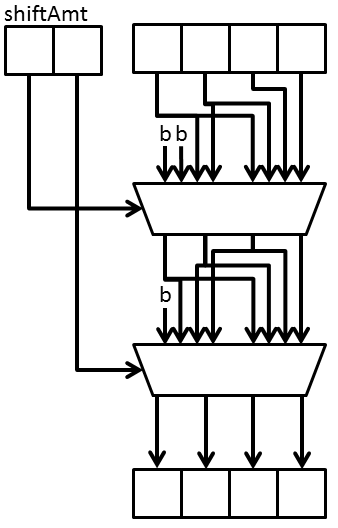
\includegraphics[width=0.7\linewidth]{VariableShifter.png}
	\caption{Variable Shifting by a Register Value}
	\label{fig:variable_shifter}
\end{subfigure}
\caption{Different Types of Shifters}
\end{figure}

\section{Getting Started}
\subsection{How to Download the Source Code}
컴퓨터 구조 과목에서 사용하게 될 모든 실습은 Lab0에서도 언급되었듯이 svn 서버를 통해 관리됩니다.
Lab1의 실습 코드를 받으시기 위해서는 다음 그림과 같이 수업 홈페이지에 올라와 있는 \texttt{add-lab1.sh} 스크립트를
실행해 주시면 됩니다. 그림의 test 부분에는 lab 0에서 사용한 본인의 ID를 적으셔야 합니다.
첫번째로 암호를 물어보는 상태에서는 강의 자료 다운로드 시 사용하는 비밀번호를 입력하세요.

\begin{Verbatim}[frame=single]
   $ ./add-lab1.sh YOUR_ID
   Getting source codes for
   archi16@hyewon.snu.ac.kr's password:
\end{Verbatim}

\noindent 다음과 같이 두번째로 암호를 물어보는 상태에서는 조교에게 제출한 본인의 ID에 맞는 암호를 입력하세요.


\begin{Verbatim}[frame=single]
    Checking in initial repository
    Authentication realm: <svn://hyewon.snu.ac.kr:3690> 2016 Computer Architecture
    Password for 'YOUR_ID':
\end{Verbatim}

\ \\ \noindent아래의 메시지가 보이면 실습 코드 다운이 완료된 것입니다.
\begin{Verbatim}[frame=single]
    ...
    Adding initial directoires to repository
    ...
    Checking in initial repository
    ...
    Transmitting file data ........
    Committed revision XX
\end{Verbatim}

\subsection{Directory Structure of Lab1}
Lab1 실습의 디렉토리 구조는 다음과 같습니다.

\begin{figure*}[!h]
\begin{verbatim}
lab1/
    build/
    lib/
        TestBench.bsv
        ...
    src/
        BarrelShifterRight.bsv
        Multiplexer.bsv
        Makefile
\end{verbatim}
\caption{Directory structure of Lab1}
\label{fig:files}
\end{figure*}

\begin{description}
\item [\texttt{build}]\hfill \ \\ 컴파일 시 생성되는 파일들이 위치하는 폴더입니다.

\item [\texttt{lib}]\hfill \ \\ 실습에 사용되는 library 파일들이 위치하는 폴더입니다.

\item [\texttt{lib/TestBench.bsv}]\hfill \ \\ Multiplexer 및 barrel shifter 모듈을 시뮬레이션 할 수 있는 Bluespec 코드
입니다.


\item [\texttt{src/Multiplexer.bsv}]\hfill \ \\ 삼항연산자를 사용하는 multiplexer 함수들을 가지고 있습니다.
이 파일을 수정하여 multiplexer 관련 숙제를 진행합니다.

\item [\texttt{src/BarrelShifterRight.bsv}]\hfill \ \\ `$>>$' 연산자를 사용하는 기본적인 barrel shifter 초기 모듈을
가지고 있습니다. 이 파일을 수정하여 barrel shifter 관련 숙제를 진행합니다.

\item [\texttt{src/Makefile}]\hfill \ \\ Lab 1 코드의 컴파일 관련 명령 및 세부적인 사항이 정의되어 있습니다. \textit{make} 명령을 통해
bluespec 코드의 컴파일 가능하게 해줍니다.

\end{description}

\subsection{How to Test the Design}
실습에서 제공되는 test-bench는 여러분이 구현할 multiplexer 및 combinational barrel-shifter의 동작을 확인합니다.
먼저 모듈의 컴파일은
\begin{verbatim}
    $./make  or  $./make mul  or  $./make rl  or  $./make ra
\end{verbatim}
와 같은 명령을 통해 수행할 수 있습니다.
각각의 컴파일을 통해 생성된 실행파일을 실행하는 것으로 여러분이 구현한 모듈의 동작을 확인할 수 있습니다.
컴파일 및 테스트에 대한 자세한 내용은 연관된 Exercise에 설명되어 있습니다.

\subsection{How to Submit Your Design}
다음과 같이 lab 1 폴더에서 \textit{svn commit} 명령을 수행하면 수정된 파일들이 제출됩니다.
이때에도 조교에게 제출한 본인의 ID에 맞는 암호를 입력하세요.
마지막 줄의 메시지가 나타나면 숙제 제출이 정상적으로 완료되었음을 나타냅니다.

\begin{Verbatim}[frame=single]
    Log message unchanged or not specified
    (a)bort, (c)ontinue, (e)dit:
    c
    Authentication realm: <svn://hyewon.snu.ac.kr:3690> 2016 Computer Architecture
    Password for 'YOUR_ID':
    Sending   src/Multiplexer.bsv
    Transmitting file data .
    Committed revision 54.
\end{Verbatim}

\section{Building a Barrel Shifter in Bluespec}

\subsection{Multiplexers}

The first step in constructing or barrel shifter is to build a basic
multiplexer from gates. Let's first examine Multiplexer.bsv.

\begin{verbatim}
function Bit#(1) multiplexer1(Bit#(1) sel, Bit#(1) a, Bit#(1) b);
\end{verbatim}

This begins a definition of a new function called multiplexer1. This
multiplexer function takes several arguments which will be used in defining
the behavior of the multiplexer. This multiplexer operates on single bit values,
the concrete type \verb|Bit#(1)|. Later we will learn how to implement polymorphic
functions, which can handle arguments of any width.

This function uses C-like constructs in its definition. Simple code, such as
the multiplexer can be defined at the high level without implementation
penalty. However, because hardware compilation is a dificult, multi-dimensional
problem, tools are limited in the kinds of optimizations that they can do. As we
shall see later with the high-level barrel shifter, high-level constructs can
sometimes result in inefficient hardware. As a result, even complicated designs
like processors may be implemented at the gate-level (or even transistor-level)
to achieve maximum performance.
\begin{verbatim}
  return (sel == 0)? a: b;
endfunction
\end{verbatim}
The \texttt{return} statement, which constitutes the entire function, takes two input and
selects between them using \texttt{sel}. The \texttt{endfunction} keyword completes the
definition of our multiplexer function. You should be able to compile the module.

\noindent \paragraph{\bf Exercise 1 (10 Points):} Using the and, or, and not gates, re-implement the
function \verb|multiplexer1| in Multiplexer.bsv. How many gates are needed?
(The required functions, called \texttt{and1}, \texttt{or1} and \texttt{not1},
respectively, are provided)

\subsection{Static Elaboration}

The data path width of the SMIPS processor is 32 bits, so we will need
multiplexers that are larger than a single bit. However, writing the code to
manually instantiate 32 single-bit multiplexers to form a 32-bit multiplexer
would be tedious. Fortunately, Bluespec provides constructs for powerful static
elaboration which we can use to make writing the code easier. Static elaboration
refers to the process by which the Bluespec compiler evaluates expressions at
compile time, using the results to generate the hardware. Static elaboration
can be used to express extremely flexible designs in only a few lines of code.

In Bluespec we can use bracket notation (\verb|[]|) to index individual bits in
a wider Bit type, for example \verb|bitVector[1]|. We can use a for-loop to
copy many lines of code which have the same form. For example, to aggregate the
multiplexer1 function to form a larger multiplexer, we could write:

\begin{verbatim}
function Bit#(32) multiplexer32(Bit#(1) sel, Bit#(32) a, Bit#(32) b);
  Bit#(32) aggregate;
  for(Integer i = 0; i < 32; i = i + 1)
    aggregate[i] = multiplexer1(sel, a[i], b[i]);
  return aggregate;
endfunction
\end{verbatim}

The Bluespec compiler, during its static elaboration phase, will replace this
for-loop with its fully unrolled version.

\begin{verbatim}
aggregate[0] = multiplexer1(sel, a[0], b[0]);
aggregate[1] = multiplexer1(sel, a[1], b[1]);
aggregate[2] = multiplexer1(sel, a[2], b[2]);
...
aggregate[31] = multiplexer1(sel, a[31], b[31]);
\end{verbatim}

\noindent \paragraph{\bf Exercise 2 (10 Point):} Complete the implementation of the function
\verb|multiplexer32| in Multiplexer.bsv using for-loops (in other words, copy
the above code).

Check the correctness of the code by running the multiplexer testbench:

\begin{verbatim}
$ make mul
$ ./simMul
\end{verbatim}

\subsection{Polymorphism and Higher-order Constructors}

So far, we have implemented two versions of the multiplexer function, but it is
easy to imagine needing an n-bit multiplexer. It would be nice if we did not
have to completely re-implement the multiplexer whenever we want to use a
different width. Using the for-loops introduced in the previous section, our
multiplexer code is already somewhat parametric because we use a constant size
and the same type throughout. We can do better by giving a name (\texttt{N}) to
the size of the multiplexer using \texttt{typedef}.  Our new multiplexer code looks like:

\begin{verbatim}
typedef 32 N;
function Bit#(N) multiplexerN(Bit#(1) sel, Bit#(N) a, Bit#(N) b);
  Bit#(N) aggregate;
  for(Integer i = 0; i < valueOf(N); i = i + 1)
    aggregate[i] = multiplexer1(sel, a[i], b[i]);
  return aggregate;
endfunction
\end{verbatim}

The \texttt{typedef} gives us the ability to change the size of our multiplexer
at will. The \texttt{valueOf} function introduces a small subtlety in our code:
\texttt{N} is not an Integer but a \emph{numeric type} and must be converted to
an Integer before being used in an expression. Even though it is improved, our
implementation is still missing some flexibility. All instantiations of the
multiplexer must have the same type, and we still have to produce new code each
time we want a new multiplexer. However, in Bluespec, we can further
parameterize the module to allow different instantiations to have
instantiation-specific parameters. This sort of module is polymorphic, the
implementation of the hardware changes automatically based on compile time
configuration. Polymorphism is the essence of design-space exploration in
Bluespec.

The truly polymorphic multiplexer will be as follows:

\begin{verbatim}
//typedef 32 N; // Not needed
function Bit#(n) multiplexer_n(Bit#(1) sel, Bit#(n) a, Bit#(n) b);
\end{verbatim}

The variable \texttt{n} represents the width of the multiplexer, replacing the
concrete value \texttt{N} (=32). In Bluespec \emph{type variables} (\texttt{n})
start with a lower case whereas concrete types (\texttt{N}) start with an upper
case.

\noindent \paragraph{\bf Exercise 3 (10 Points):} Complete the definition of the function
\verb|multiplexer_n|. Verify that this function is correct by replacing the
original definition of multiplexer32 to only have:
\\ \verb|   return multiplexer_n(sel, a, b);|.
\\ This redefinition allows the test benches to test
your new implementation without modication.

\subsection{Building a Barrel Shifter}

We will now use the multiplexers that we implemented in the previous section to
build a logical barrel shifter. To build this shifter we need a logarithmic
number of multiplexers. At each stage, we will shift over twice as many bits as
the previous stage, based on the control value, as shown in
Figure~\ref{fig:variable_shifter}.

The implementation for the barrel-shifters can be found in
BarrelShifterRight.bsv.  Notice that all the barrel-shifters are declared as
modules, as opposed to as functions. This is a subtle, but important
distinction. In Bluespec, functions are inlined by the compiler automatically,
while modules must be explicitly instantiated using the '\verb|<-|' notation.
If we made the barrel shifter a function, using it in multiple locations would
instantiate multiple barrel shifters. One purpose of this lab was to build
shift algorithms that share as much logic as possible, so we make the barrel
shifter a module.

\sloppy
There are three modules inside BarrelShifterRight.bsv,
\texttt{mkBarrelShifterRight}, \texttt{mkBarrelShifterRightLogical}, and
\texttt{mkBarrelShifterRightArithmetic}. All three modules contain a method
named \texttt{rightShift}, which implements the right shift. Notice that
\texttt{rightShift} in \texttt{mkBarrelShifterRight} takes three arguments
while \texttt{rightShift} in the others take only two. The third argument,
\texttt{shiftValue}, specifies whether 0 or 1 is shifted in.  In the logical
barrel shifter, we always shift in 0 to the high-order bits. The arithmetic
right shift preserves sign, so we need to examine the two's complement sign
(high-order) bit and the shift mode to fill in the correct bits. The
\texttt{mkBarrelShifterRightLogical} and
\texttt{mkBarrelShifterRightArithmetic} should instantiate the basic
\texttt{mkBarrelShifterRight}, and should supply the appropriate arguments to
the \texttt{shiftRight} in \texttt{mkBarrelShifterRight} to implement the
logical and arithmetic shifters, respectively.


\sloppy
\noindent \paragraph{\bf Exercise 4 (20 Points):}
Complete an implementation of the 32-bit barrel shifter in
\texttt{mkBarrelShifterRight}. Use exactly five 32-bit multiplexers in a
for-loop.
With the \texttt{mkBarrelShifterRight}, complete an implementation of the 32-bit logical shifter in
\verb|mkBarrelShifterRightLogical|, using \verb|mkBarrelShifterRight| that you
have implemented already.
Check the correctness of the code by running the logical shifter testbench:

\begin{verbatim}
$ make rl
$ ./simRl
\end{verbatim}

\sloppy
\noindent \paragraph{\bf Exercise 5 (10 Points):} Complete an implementation of
the 32-bit arithmetic shifter in \verb|mkBarrelShifterRightArithmetic|, using \verb|mkBarrelShifterRight| that you
have implemented already.

Check the correctness of the code by running the arithmetic shifter testbench:

\begin{verbatim}
$ make ra
$ ./simRa
\end{verbatim}

\end{document}
